\documentclass[xelatex,aspectratio=169]{beamer}

\hfuzz=10pt
\vfuzz=10pt

% Theme
\usetheme{htw}
\setbeamertemplate{navigation symbols}{}
\setbeamertemplate{theorems}[numbered]
\setbeamercovered{transparent}

%\logo{
\includegraphics[height=0.5cm]{HTWD_color.png}}

% Packages
\usepackage{polyglossia}
\setmainlanguage{german}
\setotherlanguage{english}

\usepackage[bigfiles]{pdfbase}
\ExplSyntaxOn
\NewDocumentCommand\embedvideo{smm}{
\group_begin:
\leavevmode
\tl_if_exist:cTF{file_\file_mdfive_hash:n{#3}}{
  \tl_set_eq:Nc\video{file_\file_mdfive_hash:n{#3}}
}{
  \IfFileExists{#3}{}{\GenericError{}{File~`#3'~not~found}{}{}}
  \pbs_pdfobj:nnn{}{fstream}{{}{#3}}
  \pbs_pdfobj:nnn{}{dict}{
    /Type/Filespec/F~(#3)/UF~(#3)
    /EF~<</F~\pbs_pdflastobj:>>
  }
  \tl_set:Nx\video{\pbs_pdflastobj:}
  \tl_gset_eq:cN{file_\file_mdfive_hash:n{#3}}\video
}
%
\pbs_pdfobj:nnn{}{dict}{
  /Type/RichMediaInstance/Subtype/Video
  /Asset~\video
  /Params~<</FlashVars (
  source=#3&
  skin=SkinOverAllNoFullNoCaption.swf&
  skinAutoHide=true&
  skinBackgroundColor=0x5F5F5F&
  skinBackgroundAlpha=0.75
  )>>
}
%
\pbs_pdfobj:nnn{}{dict}{
/Type/RichMediaConfiguration/Subtype/Video
/Instances~[\pbs_pdflastobj:]
}
%
\pbs_pdfobj:nnn{}{dict}{
/Type/RichMediaContent
/Assets~<<
/Names~[(#3)~\video]
>>
/Configurations~[\pbs_pdflastobj:]
}
\tl_set:Nx\rmcontent{\pbs_pdflastobj:}
%
\pbs_pdfobj:nnn{}{dict}{
  /Activation~<<
  /Condition/\IfBooleanTF{#1}{PV}{XA}
  /Presentation~<</Style/Embedded>>
  >>
  /Deactivation~<</Condition/PI>>
}
%
\hbox_set:Nn\l_tmpa_box{#2}
\tl_set:Nx\l_box_wd_tl{\dim_use:N\box_wd:N\l_tmpa_box}
\tl_set:Nx\l_box_ht_tl{\dim_use:N\box_ht:N\l_tmpa_box}
\tl_set:Nx\l_box_dp_tl{\dim_use:N\box_dp:N\l_tmpa_box}
\pbs_pdfxform:nnnnn{1}{1}{}{}{\l_tmpa_box}
%
\pbs_pdfannot:nnnn{\l_box_wd_tl}{\l_box_ht_tl}{\l_box_dp_tl}{
  /Subtype/RichMedia
  /BS~<</W~0/S/S>>
  /Contents~(embedded~video~file:#3)
  /NM~(rma:#3)
  /AP~<</N~\pbs_pdflastxform:>>
  /RichMediaSettings~\pbs_pdflastobj:
  /RichMediaContent~\rmcontent
}
\phantom{#2}
\group_end:
}
\ExplSyntaxOff


\usepackage{graphicx}
\usepackage[export]{adjustbox}
\usepackage{animate}
%\usepackage[dvipdfmx]{movie15_dvipdfmx}
\usepackage{media9}
\usepackage{tabularx}
\usepackage{colortbl}
\usepackage{booktabs}
\usepackage{makecell}
\usepackage{ltablex}
\usepackage{array}
\usepackage{multirow}
\usepackage{amsmath}
\usepackage{amsthm}
%\renewcommand{\arraystretch}{1.5}
\newcolumntype{L}[1]{>{\raggedright\let\newline\\\arraybackslash\hspace{0pt}}p{#1}}
\newcolumntype{C}[1]{>{\centering\let\newline\\\arraybackslash\hspace{0pt}}p{#1}}
\newcolumntype{R}[1]{>{\raggedleft\let\newline\\\arraybackslash\hspace{0pt}}p{#1}}
%\renewcommand\thesatz{\arabic{section}.\arabic{theorem}}
\makeatletter
\@addtoreset{theorem}{lecture}
\makeatother

\newtheorem{satz}{Satz}[section]
\newtheorem{lem}{Lemma}[section]
\newtheorem{beh}{Behauptung}[section]
\newtheorem{define}{Definition}[section]
\numberwithin{equation}{section}
\usepackage{ragged2e}
\usepackage{etoolbox}

\usepackage{color}
\usepackage{colortbl}
\definecolor{hellgrau}{rgb}{0.85,0.85,0.85}
\definecolor{hellrot}{rgb}{1,0.7,0.7}

\usepackage{tikz}
\usetikzlibrary{shapes,arrows.meta,calc,arrows,positioning,patterns,tikzmark}
%\usepackage{tikz-uml}
\usepackage{pgfplots}  % for elliptic curves (part 8)
\pgfplotsset{compat=1.18}
\usepackage{pgffor}
\usepackage{pgfmath-xfp}
\tikzset{>=latex}
\tikzset{
  invisible/.style={opacity=0},
  visible on/.style={alt={#1{}{invisible}}},
  alt/.code args={<#1>#2#3}{%
      \alt<#1>{\pgfkeysalso{#2}}{\pgfkeysalso{#3}} % \pgfkeysalso doesn't change the path
    },
}

\usepackage{paralist}

\usepackage{url}
\def\UrlBreaks{\do\/\do-}
\PassOptionsToPackage{hyphens}{url}\usepackage{hyperref}

\usepackage[normalem]{ulem} % gestrichelte Unterstreichung (\dashuline{})
\usepackage{cancel}

\makeatletter
\renewcommand{\itemize}[1][]{%
  \beamer@ifempty{#1}{}{\def\beamer@defaultospec{#1}}%
  \ifnum \@itemdepth >2\relax\@toodeep\else
    \advance\@itemdepth\@ne
    \beamer@computepref\@itemdepth% sets \beameritemnestingprefix
    \usebeamerfont{itemize/enumerate \beameritemnestingprefix body}%
    \usebeamercolor[fg]{itemize/enumerate \beameritemnestingprefix body}%
    \usebeamertemplate{itemize/enumerate \beameritemnestingprefix body begin}%
    \list
    {\usebeamertemplate{itemize \beameritemnestingprefix item}}
    {\def\makelabel##1{%
        {%
            \hss\llap{{%
                  \usebeamerfont*{itemize \beameritemnestingprefix item}%
                  \usebeamercolor[fg]{itemize \beameritemnestingprefix item}##1}}%
          }%
      }%
    }
  \fi%
  \beamer@cramped%
  \justifying% NEW
  %\raggedright% ORIGINAL
  \beamer@firstlineitemizeunskip%
}
\makeatother

\apptocmd{\frame}{}{\justifying}{}

\renewcommand\theadfont{\bfseries\sffamily}
\usepackage{ragged2e}
\usepackage{newpxtext}

\setsansfont{texgyreheros}[
  Scale=MatchLowercase,
  UprightFont=*-regular,
  BoldFont=*-bold,
  ItalicFont=*-italic,
  BoldItalicFont=*-bolditalic,
]

% Title
\usepackage[usetransparent=false]{svg}
% Import references
\usepackage[backend=biber,style=numeric,sorting=none]{biblatex}
\addbibresource{references.bib}

%\AtBeginSection[]{
%  \begin{frame}
%    \vfill
%    \centering
%    \begin{beamercolorbox}[sep=8pt,center,shadow=true,rounded=true]{title}
%      \usebeamerfont{title}\thesection.~\secname\par%
%    \end{beamercolorbox}
%    \vfill
%  \end{frame}
%}

\makeatletter
\newenvironment{noheadline}{
  \setbeamertemplate{headline}{}
  \addtobeamertemplate{frametitle}{\vspace*{-0.9\baselineskip}}{}
}{}
\makeatother


\usepackage{xcolor}
\usepackage{algorithm}
\usepackage[linesnumbered,ruled,lined,commentsnumbered,algo2e,ngerman,ngermankw]{algorithm2e}
\usepackage{algorithmic}
\usepackage{caption}
\usepackage[newfloat]{minted}
\captionsetup[listing]{position=top}
\definecolor{mintedbg}{HTML}{282828}
\setminted{
  breaklines=true,
  bgcolor=mintedbg,
  style=monokai,
  formatcom=\color{white}
}
\usepackage{etoolbox}
\makeatletter
% replace \medskip before and after the box with nothing, i.e., remove it
\patchcmd{\minted@colorbg}{\medskip}{}{}{}
\patchcmd{\endminted@colorbg}{\medskip}{}{}{}
\makeatother

\renewcommand{\theFancyVerbLine}{\textcolor{black}{\arabic{FancyVerbLine}}}

\usepackage{pifont}
\newcommand{\cmark}{\ding{51}}%
\newcommand{\xmark}{\ding{55}}%

\newenvironment{changemargin}[2]{%
  \begin{list}{}{%
      \setlength{\topsep}{0pt}%
      \setlength{\leftmargin}{#1}%
      \setlength{\rightmargin}{#2}%
      \setlength{\listparindent}{\parindent}%
      \setlength{\itemindent}{\parindent}%
      \setlength{\parsep}{\parskip}%
    }%
    \item[]}{\end{list}}


\usepackage{csquotes}

% Title
\title{Algorithmen}
\author{Prof. Dr. Lukas Iffländer}
\institute{HTW Dresden}
\date{}
\usepackage{svg}

% Begin document
\begin{document}

\begin{frame}{Unicode}{Motivation}
    \centering
    
\includegraphics[height=.8\textheight]{img/codierung_scheisse.png}
\end{frame}

\begin{frame}{Unicode}{Entwicklung}
    \begin{itemize}
        \item Entwicklung durch das Unicode Konsortium
        \item (Codierter) Zeichensatz mit erweiterbarem Zeichenvorrat
              \begin{itemize}
                  \item Unicode 1.0 (1991): ~7000 Zeichen
                  \item Unicode 6.0 (2010): ~109.000 Zeichen
                  \item Unicode 12.0 (2019): ~137.000 Zeichen
                  \item Unicode 15.0 (2022): ~149.000 Zeichen
              \end{itemize}
    \end{itemize}
    \begin{block}{Motto}
        Unicode provides a unique number for every character, \\
        no matter what the platform, \\
        no matter what the program, \\
        no matter what the language.
    \end{block}
\end{frame}

\begin{frame}{Unicode}{Anteil der Zeichenkodierungen für Webseiten}
    \begin{tabular}{lcccccccccc}
        \toprule
        in Prozent          & 2010 & 2011 & 2012 & 2013 & 2014 & 2015 & 2016 & 2017 & 2018 & 2019 \\
        \midrule
        \textbf{UTF-8}      & 50.6 & 59.8 & 68.0 & 74.7 & 78.7 & 82.3 & 86.0 & 88.2 & 90.5 & 92.8 \\
        \textbf{ISO-8859-1} & 28.6 & 22.0 & 17.2 & 13.5 & 10.8 & 9.3  & 6.9  & 5.5  & 4.3  & 3.6  \\
        \textbf{US-ASCII}   & 0.2  & 0.1  & 0.1  & 0.1  & 0.1  & 0.1  & <0.1 & <0.1 & <0.1 & <0.1 \\
        \bottomrule
    \end{tabular}
\end{frame}


\begin{frame}{Unicode}{Verfahren -- Planes I}
    \begin{itemize}
        \item Code Space wird 17 gleich große Ebenen (Planes) unterteilt
        \item Jede Plane hat 65.536 Codepunkte ($2^{16}$)
        \item Mit einer vierstelligen Hexadezimalzahl können alle code points innerhalb einer Plane adressiert werden
    \end{itemize}
    \centering
    \begin{tabular}{lcl}
        \toprule
        Plane & Name                                      & Code Range           \\
        \midrule
        0     & Basic Multilingual Plane (BMP)            & U+0000 -- U+FFFF     \\
        1     & Supplementary Multilingual Plane (SMP)    & U+10000 -- U+1FFFF   \\
        2     & Supplementary Ideographic Plane (SIP)     & U+20000 -- U+2FFFF   \\
        3     & Tertiary Ideographic Plane (TIP)          & U+30000 -- U+3FFFF   \\
        5-13  & Unassigned                                & --                   \\
        14    & Supplementary Special-purpose Plane (SSP) & U+E0000 -- U+EFFFF   \\
        15    & Supplementary Private Use Area-A (PUA-A)  & U+F0000 -- U+FFFFF   \\
        16    & Supplementary Private Use Area-B (PUA-B)  & U+100000 -- U+10FFFF \\
        \bottomrule
    \end{tabular}
\end{frame}
\begin{frame}{Unicode}{Verfahren -- Planes II}
    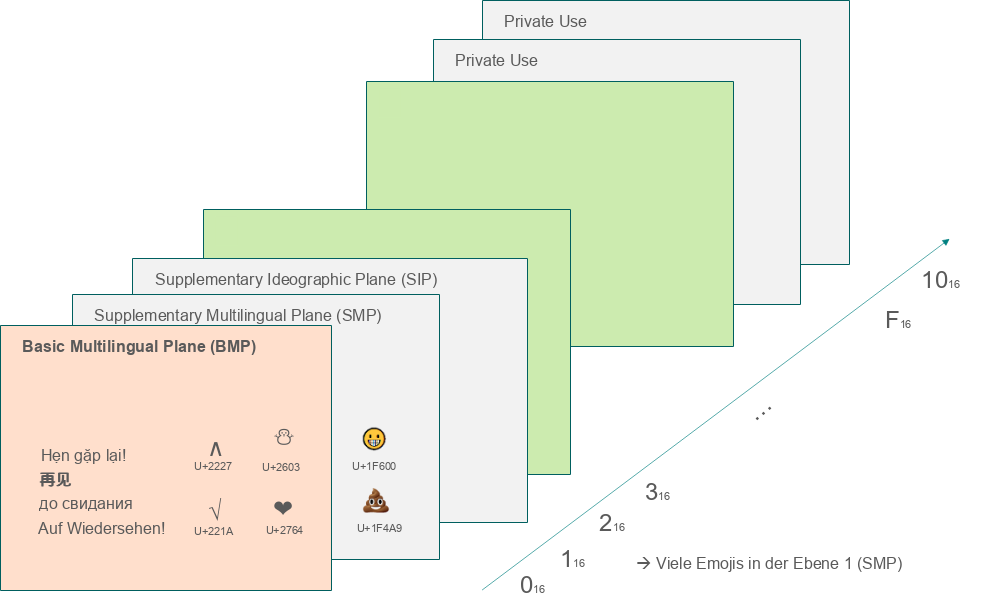
\includegraphics[height=.8\textheight]{img/codierung_planes.png}
\end{frame}

\begin{frame}{Basic Multilingual Plane (BMP)}
    \centering
    \setlength{\tabcolsep}{1em}
    \begin{tabular}{lcccccccccccccccc}
        \toprule
                        & \textbf{0}                                            & \textbf{1}                         & \textbf{2}                    & \textbf{3}                               & \textbf{4} & \textbf{5} & \textbf{6} & \textbf{7} & \textbf{8} & \textbf{9} & \textbf{A} & \textbf{B} & \textbf{C} & \textbf{D} & \textbf{E} & \textbf{F} \\
        \midrule
        \textbf{00}     & \multicolumn{2}{|c}{C0}                               & \multicolumn{6}{|c}{Basic Latin}   & \multicolumn{2}{|c}{C1}       & \multicolumn{6}{|c|}{Latin 1 Supplement}                                                                                                                                                             \\
        \textbf{01}     &                                                                                                                                                                                                                                                                                                                                   \\
        \textbf{\ldots} &                                                                                                                                                                                                                                                                                                                                   \\
        \textbf{20}     & \multicolumn{7}{|c}{General Punctation}               & \multicolumn{3}{|c}{Subs./Supers.} & \multicolumn{3}{|c}{Currency} & \multicolumn{3}{|c|}{Diac. Symbs.}                                                                                                                                                                   \\
        \textbf{\ldots} &                                                                                                                                                                                                                                                                                                                                   \\
        \textbf{FF}     & \multicolumn{16}{|c| }{Halfwidth and Fullwidth Forms}                                                                                                                                                                                                                                                                             \\
        \bottomrule
    \end{tabular}

\end{frame}

\begin{frame}{Unicode}{Unicode Character Encoding}
    \begin{alertblock}{Frage}
        Wie stellen wir das jetzt im Dualsystem dar?
    \end{alertblock}
    \begin{block}{Begrenzungen}
        \begin{itemize}
            \item Mindestens 17 Planes
            \item Jede Plane hat 65.536 Codepunkte ($2^{16}$)
            \item Wir brauchen also mindestens 17*65.536 = 1.048.576 Codepunkte
            \item Das sind 20 Bit
        \end{itemize}
    \end{block}

\end{frame}

% End document
\end{document}